\documentclass[a4paper,12pt]{article}
\usepackage{url}
\usepackage{listings}
\usepackage{color}
\usepackage{graphicx}
\usepackage{hyperref}
\usepackage{booktabs}
\definecolor{dkgreen}{rgb}{0,0.6,0}
\definecolor{gray}{rgb}{0.5,0.5,0.5}
\definecolor{mauve}{rgb}{0.58,0,0.82}
%dummy-commit


\lstset{frame=tb,
	language=C++,
	aboveskip=3mm,
	belowskip=3mm,
	showstringspaces=false,
	columns=flexible,
	basicstyle={\small\ttfamily},
	numbers=none,
	numberstyle=\tiny\color{gray},
	keywordstyle=\color{blue},
	commentstyle=\color{dkgreen},
	stringstyle=\color{mauve},
	breaklines=true,
	breakatwhitespace=true,
	tabsize=3
}
\begin{document}
	
	\title{CS-224 Object Oriented Programming and Design Methodologies }
	\author{Spring 2022}
	\date{Homework 1}
	\maketitle
	\section{Submission Policy}
	You need to submit this homework on  {\color{blue}28th January at 8pm}, on LMS. Late submissions are allowed until {\color{red} 30th January 11:59pm}, which will be penalized by 20\%. Your work will not be accepted once the submission is closed on LMS.
	
	\section{Guidelines}
		Some important guidelines about the homework are as following:
	\begin{itemize}
		\item You need to do this homework alone

		\item You need to follow the best programming practices as given in the accompanying document and it is also present on LMS. Failure in doing so will have your marks deducted.
		\item Submit assignment on time; late submissions will not be accepted.
		\item Some assignments will require you to submit multiple files. Always Zip and send them.
		\item It is better to submit incomplete assignment than none at all.
		\item It is better to submit the work that you have done yourself than what you have plagiarized.
		\item It is strongly advised that you start working on the assignment the day you get it. Assignments WILL take time.
		\item Every assignment you submit should be a single zipped file containing all the other files. Suppose your name is John Doe and your id is 0022 so the name of the submitted file should be JohnDoe0022.zip
		\item DO NOT send your assignment to your instructor, if you do I will just mark your assignment as ZERO for not following clear instructions.
		\item You can be called in for Viva for any assignment that you submit
	\end{itemize}
	
	\newpage
	
	\section{Legend of SeePlusia}

	Prince Lazy has been captured by an evil wizard. You are Zeldana, a female warrior who takes it upon
	yourself to rescue the prince and return him to his family. You go off on a quest through the dangerous
	world of SeePlusia to search for the four mythical crystals of Objectos. Together the crystals will give
	you the power to defeat the wizard and rescue Prince Lazy.
	The world of SeePlusia is shown in Fig. \ref{fig:assests}. It shows the different locations in the world. The direction of travel between locations is given by an arrow and the number of apples required to travel from one location to other are also shown.
	
	The rules of the game of Legend of SeePlusia are as follows.
\begin{itemize}
	\item You begin at Enchanted Forest on the first day with 20 apples.
	\item You have to save Prince Lazy who is held captive at Wizard's Castle.
	\item At each location you can only go in one of four directions: north, south, east, west.
	\item If a direction is not shown on the map, it's an invalid move, e.g. north from
	Marsh of the Undead. An invalid move uses up the move and consumes one apple.
	\item A valid move consumes the number of apples as drawn on the arrow, e.g. to travel from Enchanted Forest to Wampire Cove, three apples are consumed.
	\item Before rescuing the prince, you have to collect all four objectos crystals from the indicated locations.
	\item An objectos crystal is automaticaly retrieved when you arrive at its location.
	\item Once you retrieve a crystal, it is no longer present at that location.
	\item If you arrive at Sands of Quick, you slowly sink into quicksand and die and the game is Lost.
	\item You cannot move past Bridge of Death to Wizard's Castle unless you have all four crystals.
	\item You cannot move past Eisten Tunnel unless you have at least three crystals. You need 10 apples to reach Wizard's Castle from Eisten Tunnel. \textit{Call moveNorth twice to make a longer jump.}
	\item Once you reach Wizard’s Castle, the Prince is rescued and the game is Won.
	\item You can add 6 apples to your life by visiting Apples Orchard.
	\item If you run out of food before rescuing the prince, you die of starvation and the game is Lost.
\end{itemize}
	
	\section{Your Task}
	 A bare-bone implementation is given in Seeplusia folder. You can move the warrior by arrow keys, and it does some arbitrary operations to demonstrate how to use the available functions. You have to provide the implementation of \texttt{seeplusia.cpp $\Rightarrow$ makeMove (string direction)} function in accordance with the game rules given above. This function is called every time you press an arrow-key with appropriate direction provided as argument. To modularize the program, you should add other functions as well in the same file, that you call in \texttt{makeMove}.
	 
	\textit{ Note: If any rule is not clearly mentioned in the above game rules, you can implement it at your own discretion. You can make this game more fun by adding any other feature on top of the rules explained above. }
	
	\section{Game Status}
	The bottom part of screen displays the game status that shows:
	
	\begin{itemize}
		\item \textbf{Apples: } Initially it shows all the 20 apples available, as you travel the number of apples are reduced. 
		\item \textbf{Crystals: } Initially there are no crystals, but as you find one, you will increment the \texttt{nCrystalsFound}, and they will be shown next to apples.
		\item \textbf{Game State: } It displays Running, Lost or Won as per game rules. 
	\end{itemize}
	
	\section{Available Functions/Parameters}
	
	\begin{itemize}
		\item \texttt{moveEast() : } moves the warrior to East.
		\item \texttt{moveWest() : } moves the warrior to West.
		\item \texttt{moveSouth() : } moves the warrior to South.
		\item \texttt{moveNorth() : } moves the warrior to North.
		\item \texttt{applesLeft : } set it to the number of apples left.
		\item \texttt{nCrystalsFound : } set it to the number of crystals found so far.
		\item \texttt{gameState : } set it to \texttt{Running}, \texttt{Won} or \texttt{Lost}.
	\end{itemize}
	\section{Rubric}
	\begin{table}[h]
	    \centering
	    \begin{tabular}{llc}
	    \toprule
            Warnings/Errors	& The code had no warnings/errors	& 1 \\
            Comments &	The code was properly commented	& 1 \\
            Coding	& The code followed best practices guideline &	4 \\
            % Modularization &	Code is modularized in different functions	& 1\\
            Game Logic	& Game logic is fully implemented	& 4 \\
            \midrule
            Total & & 10\\
            \bottomrule
	    \end{tabular}
	    \caption{Grading Rubric}
	    \label{Grading}
	\end{table}

% 	\pagebreak
		
\begin{figure}
	\centering
	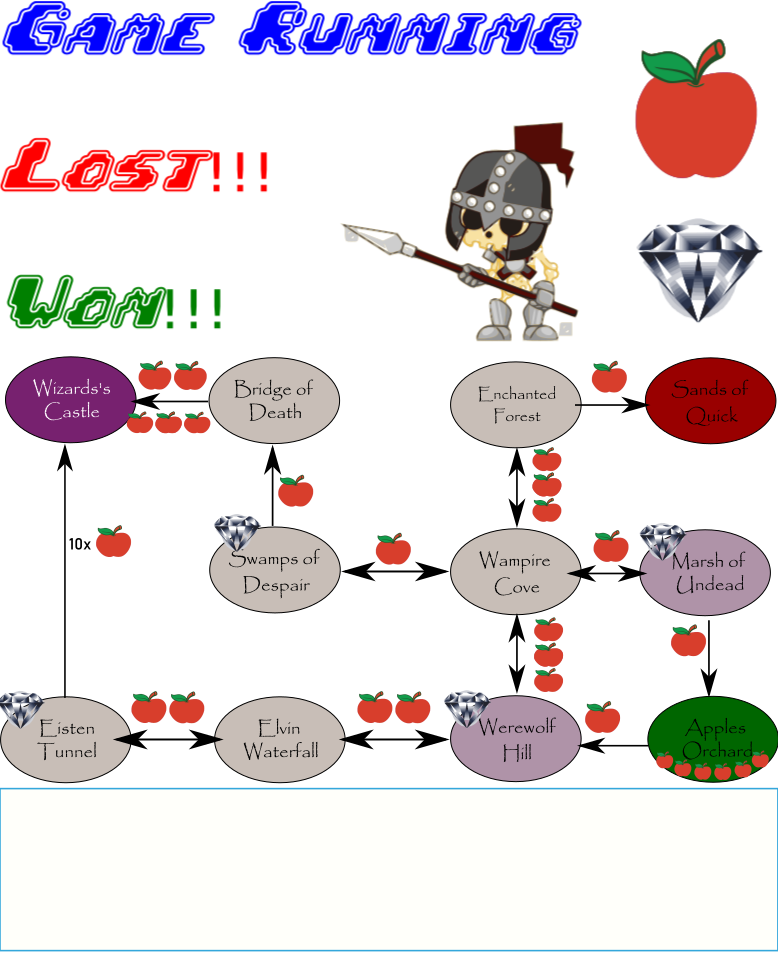
\includegraphics[trim={0 0 0 9cm},clip, width=1\linewidth]{Seeplusia/assests}
	\caption{World of Seeplusia}
	\label{fig:assests}
\end{figure}

\section{How to compile}
Open the given \texttt{Seeplusia} folder in vscode by choosing \texttt{File $\Rightarrow$ Open Folder}. The game can be run by simply pressing F5 from vscode. If due to some reason it doesn't work, then go compiling and running it from terminal, as explained in \texttt{how to compile.txt}


\section{Acknowledgement}
This assignment is adapted from the work of  \href{https://twitter.com/nav_ejaz}{Naveed Ejaz}.	
	
	
\end{document}